\section{Restrizione DNA}
\subsection{Materiali e composti utilizzati}
\paragraph{Strumentazione}
\begin{itemize}[person]
	\itemb[Vaschetta di corsa]: è un contenitore dove viene posizionato il gel di agarosio contenente i campioni ricoperto dal buffer di corsa. Possiede due elettrodi, uno positivo e uno negativo, alle estremità della vaschetta, i quali durante l'elettroforesi verranno collegati a un generatore. Questo permette la creazione del campo elettrico utile per la migrazione delle molecole.
\end{itemize}

\paragraph{Composti utilizzati}
\begin{itemize}[person]
	\itemb[Buffer 10X]: garantisce le condizioni di reazione ottimali per gli enzimi di restrizione
	\itemb[DNA]
	\itemb[\enzima{EcoR I}]: enzima di restrizione 
	\itemb[\foreignlanguage{english}{DNA ladder}]: miscela di frammenti di DNA di varie dimensioni note che, separandosi durante la corsa elettroforetica, creano una scala di valutazione per il dimensionamento approssimativo gli amplificati.
	\itemb[Agarosio]: componente base per i gel di corsa
	\itemb[TAE 50X]: tampone che viene utilizzato sia per la polimerizzazione dell'agarosio sia per il tampone di corsa. é composto da Trisacetato ed EDTA. Quest'ultimo è un chelante che sequenza ioni \ch{Mg^{2+}} presenti in soluzione per inibire l'attività degli enzimi DNAsi
	\itemb[SyberSafe]: è un colorante altamente sensibile per la visualizzazione del DNA in gel di agarosio o acrilammide. È stato formulato per essere un'alternativa meno pericolosa al bromuro di etidio che può utilizzare la luce blu o l'eccitazione UV. 
	\itemb[\foreignlanguage{english}{Sample Buffer}]: colorante per osservare la corsa dei campioni sul gel di agarosio
\end{itemize}

\subsection{Protocollo}
\subsubsection{Preparazione della reazione di digestione}
\begin{enumerate}
	\item Preparare in due \foreignlanguage{german}{Eppendorf} da \qty{1.5}{\ml} due campioni, i quali sono:
	\begin{itemize}
		\item plasmide digerito (\autoref{img:3-02})
		\begin{itemize}
			\item \qty{11.5}{\micro\litre} di \ch{H2O}
			\item \qty{10}{\micro\litre} di DNA
			\item \qty{2.5}{\micro\litre} di buffer 10X
			\item \qty{1}{\micro\litre} di \emph{EcoR I}
		\end{itemize}
		\item controllo negativo -- senza enzima (\autoref{img:3-01})
		\begin{itemize}
			\item \qty{12.5}{\micro\litre} di \ch{H2O}
			\item \qty{10}{\micro\litre} di DNA
			\item \qty{2.5}{\micro\litre} di buffer 10X
		\end{itemize}
	\end{itemize}
	\begin{Note}
		I componenti vanno aggiunti in ordine decrescente di volume per minimizzare le perdite e migliorare la miscelazione dei componenti della soluzione.
	\end{Note}
	\item Vortexare e centrifugare entrambe le soluzioni
	\item Lasciare le soluzioni a digerire per \qtyrange{1}{2}{\hour} a \qty{37}{\celsius}
\end{enumerate}

\subsubsection{Preparazione del gel di agarosio}\label{sssec:agarosio}
\begin{enumerate}
	\item Pesare con una beuta \qty{0.6}{\g} di agarosio sulla bilancia tecnica 
	\item In cilindro mettere \qty{1.6}{\ml} di TAE 50X e poi aggiungere acqua distillata fino a raggiungere il volume di \qty{80}{\ml}. Infine versare il tutto nella beuta contenete agarosio (\autoref{img:3-03})
	\item Riscaldare in microonde la soluzione preparata senza farla bollire
	\item Aspettare qualche minuto che si raffreddi oppure velocizzare il processo mettendo la beuta sotto acqua corrente (\autoref{img:3-04})
	\item Una volta raffreddata, aggiungere \qty{3}{\micro\litre} di SyberSafe e mescolare (\autoref{img:3-07})
	\item Versare la soluzione nella vaschetta (precedentemente preparata con lo scotch) e nel caso si formano delle bolle romperle (\autoref{img:3-08})
	\item Aspettare che il gel si solidifichi, dopo di ciò rimuovere il pettinino
\end{enumerate}

\subsubsection{Elettroforesi}
\begin{enumerate}
	\item Inserire la vaschetta nello strumento per la corsa elettroforetica (\autoref{img:3-12}) e ricoprirla con \qty{250}{\ml} di buffer di corsa 
	\item Aggiungere ai campioni da inserire \qty{5}{\micro\litre} di \foreignlanguage{english}{Sample Buffer}
	\item Inserire i campioni nei pozzetti (\autoref{img:3-15}), corrispondenti a:
	\begin{itemize}
		\item \qty{25}{\micro\litre} di DNA digerito
		\item \qty{25}{\micro\litre} di DNA non digerito
		\item \qty{25}{\micro\litre} di RNA totale
	\end{itemize}
	\item Nell'ultimo pozzetto, aggiungere \qty{5}{\micro\litre} di DNA \foreignlanguage{english}{ladder}, il nostro marker
	\item Impostare il voltaggio della corsa tra \qtyrange{90}{100}{\volt} e lanciare la corsa elettroforetica
	\item Una volta finita la corsa, guardare il gel agli UV, per constatare se la digestione è avvenuta
\end{enumerate}

\begingroup
	\newpage
	\newgeometry{top=.5in,bottom=.5in}
	\photo{
		\img{3-01}{\\\slz DNA\\ senza enzima}{3-01}{trim={5cm 20cm 15cm 20cm},clip}		
	}{
		\img{3-02}{\\\slz DNA\\ con enzima}{3-02}{trim={10cm 30cm 10cm 10cm},clip}
	}{
		\img{3-03}{\\\slz di agarosio\\ (prima del riscaldamento)}{3-03}{}		
	}

	\vspace{.15cm}
	\photo{
		\img{3-04}{\\\slz di agarosio\\ (dopo del riscaldamento)}{3-04}{trim={15cm 0 15cm 0},clip}		
	}{
		\img{3-07}{\\Aggiunta di SyberSafe\\\phantom{}}{3-07}{trim={5cm 20cm 5cm 0},clip}		
	}{
		\img{3-08}{\\Vaschetta piena\\\phantom{}}{3-08}{trim={5cm 10cm 5cm 10cm},clip}
	}

	\vspace{-.5cm}
	\photo{
		\begin{figure}[H]
			\captionsetup{singlelinecheck=off}
			\centering
			\begin{annotatedFigure}
				{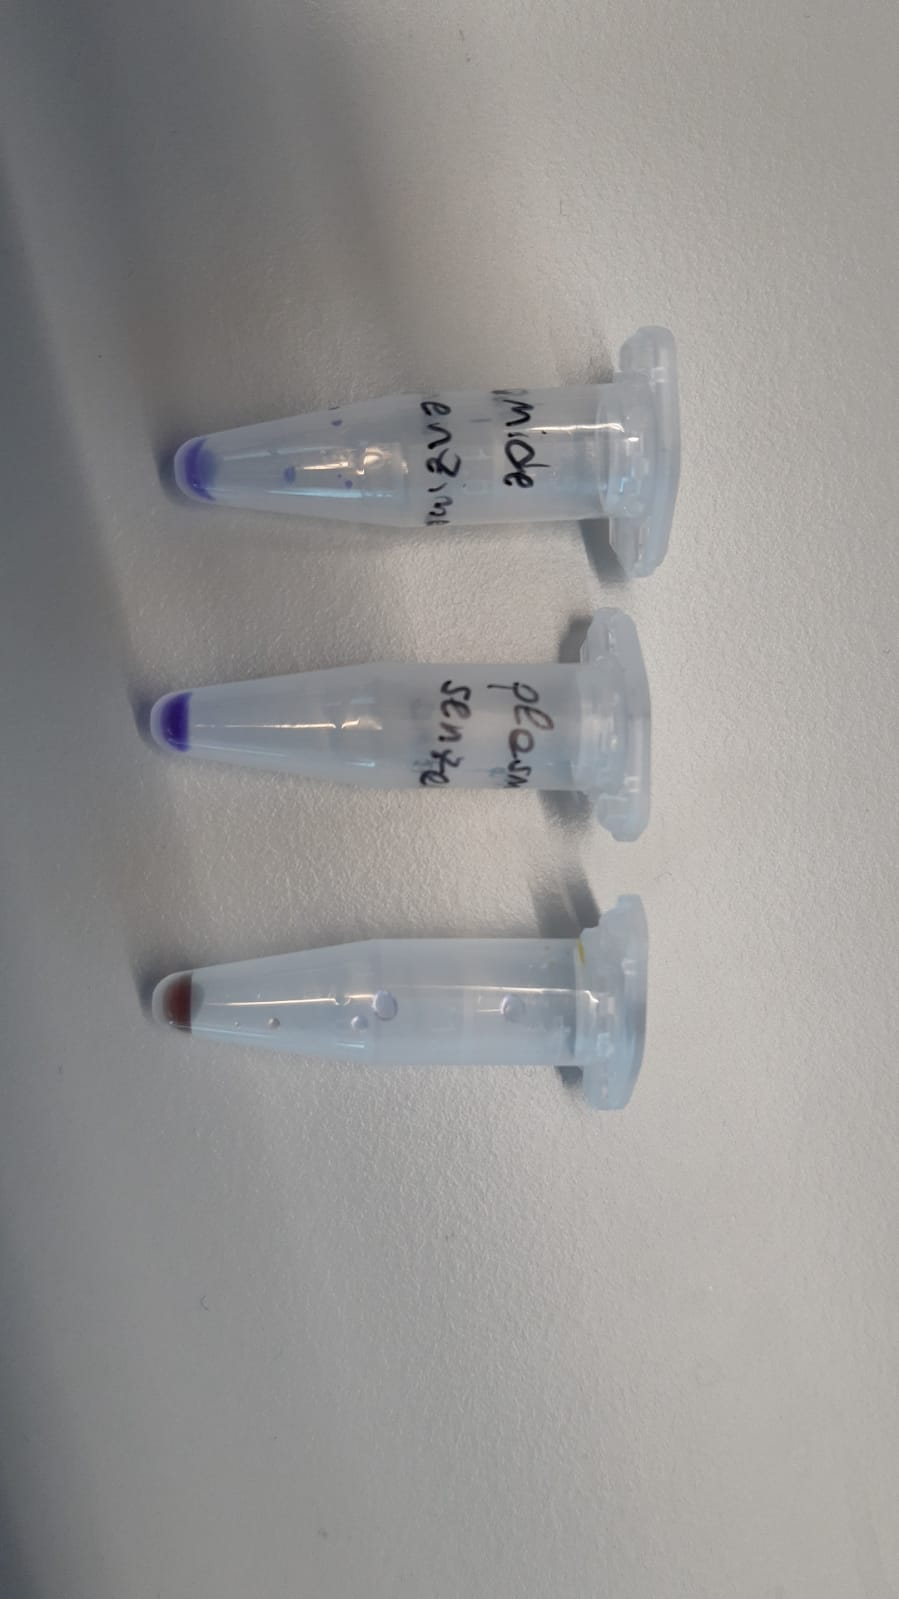
\includegraphics[
					width=4cm,
					height=6cm,
					]{3-16}
				}
				\annotatedFigureText{0.8,0.375}{black}{}{A}
				\annotatedFigureText{0.8,0.55}{black}{}{B}
				\annotatedFigureText{0.83,0.725}{black}{}{C}
			\end{annotatedFigure}
			\caption[Piastra di agarosio]{\\Campioni inseriti nei pozzetti --
			\begin{enumerate}[person,label=\Alph*]
				\item DNA con enzima
				\item DNA senza enzima
				\item RNA
			\end{enumerate}
			}\label{img:3-16}
		\end{figure}
	}{
		\img{3-12}{\\Strumento per\\ l'elettroferesi\\\phantom{}\\\phantom{}}{3-12}{}
	}{
		\begin{figure}[H]
			\captionsetup{singlelinecheck=off}
			\centering
			\begin{annotatedFigure}
				{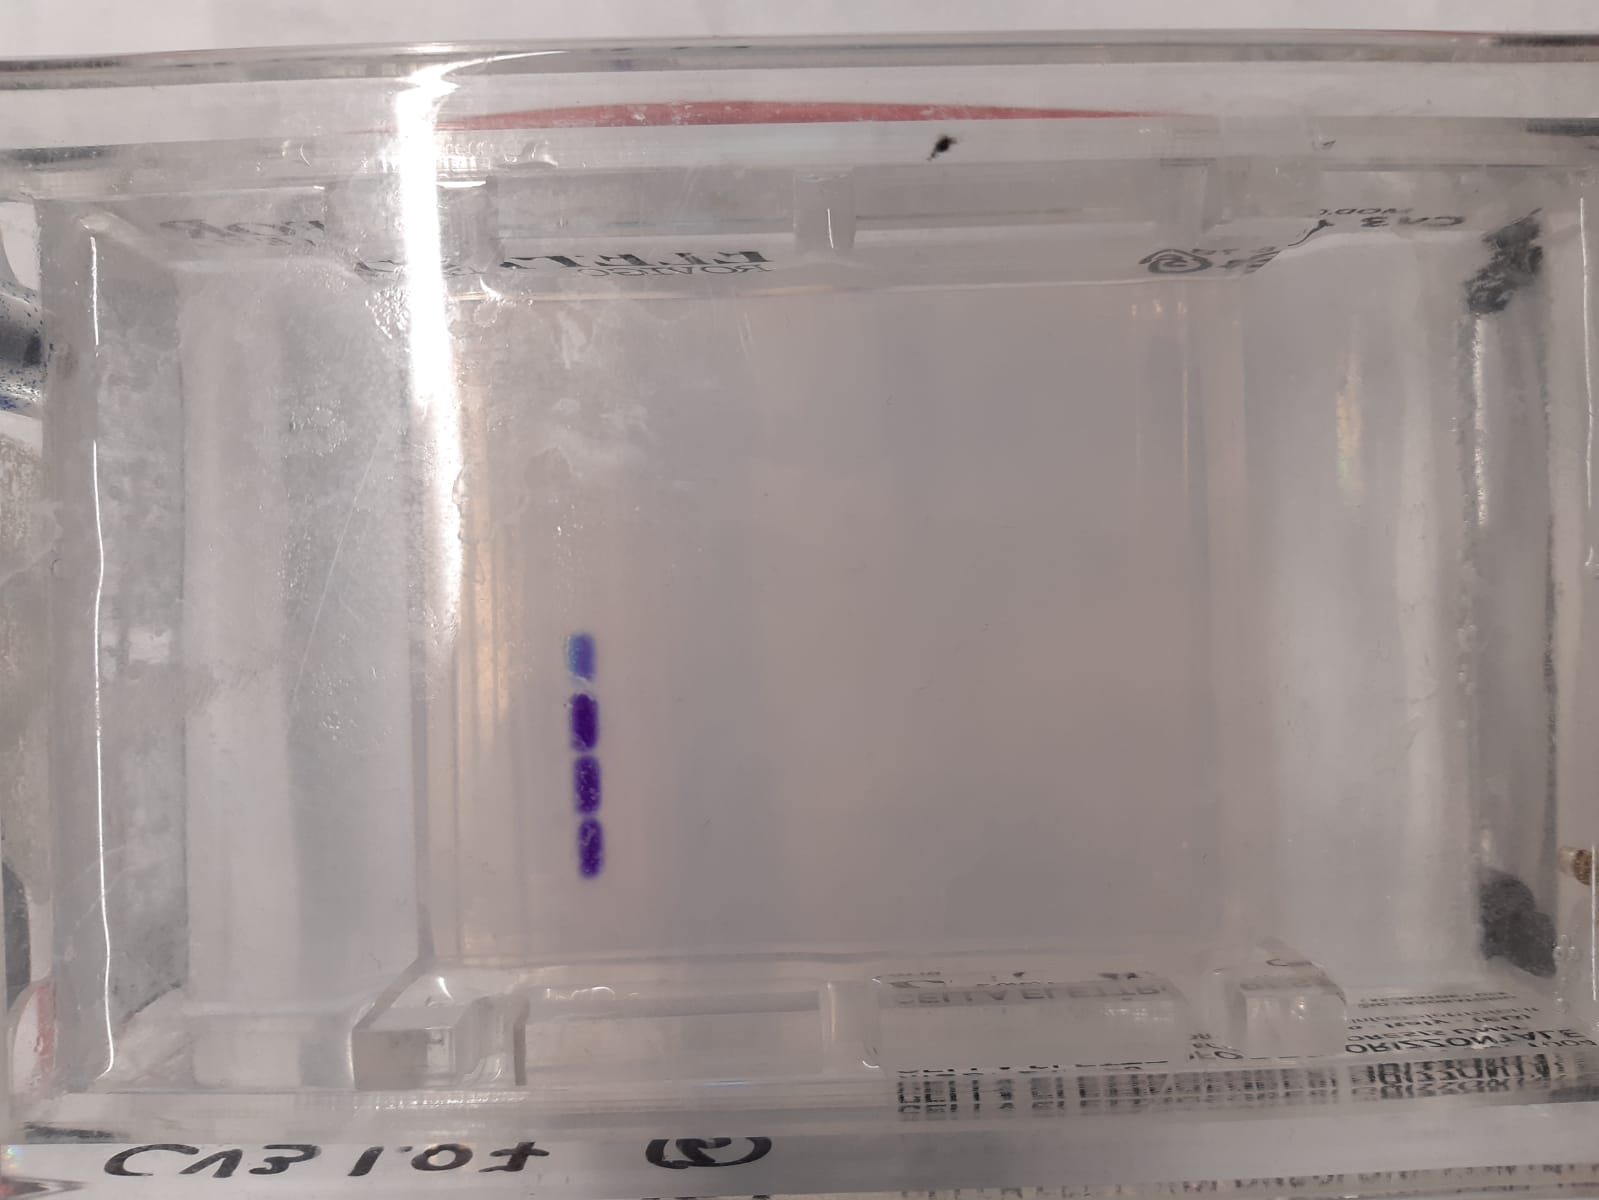
\includegraphics[
					width=4cm,
					height=6cm,
					trim={15cm 5cm 30cm 15cm},
					clip
					]{3-15}
				}
				\annotatedFigureText{0.63,0.325}{black}{}{A}
				\annotatedFigureText{0.63,0.425}{black}{}{B}
				\annotatedFigureText{0.63,0.525}{black}{}{C}
				\annotatedFigureText{0.63,0.625}{black}{}{D}
			\end{annotatedFigure}
			\caption[Piastra di agarosio]{\\Piastra di agarosio --
			\begin{enumerate}[person,label=\Alph*]
				\item DNA con enzima
				\item DNA senza enzima
				\item RNA
				\item Marker
			\end{enumerate}
			}\label{img:3-15}
		\end{figure}		
	}
\endgroup